\chapter{Desarrollo de placa de conexiones}\label{chp-03}

\lettrine[lraise=-0.1, lines=2, loversize=0.2]{P}ara simplificar todas las conexiones internas
dentro de la caja y posibilitar ciertas funciones especificadas, se crea una placa electrónica
donde se conectan todos los dispositivos. De este modo se consigue simplificar el montaje y la
posible actualización del sistema, ya que todas las conexiones internas desaparecen por completo.
Además, para favorecer el orden de los cables dentro de la caja se crea una segunda placa más básica
cuya única función es agrupar todas las conexiones existentes en la tapa. Se conocerá como placa 'Fondo'
a la placa general y placa 'Tapa' a la superior.

\section{Software utilizado. KiCAD.}

Para la realización de la placa se ha utilizado el paquete de software KiCAD. Se trata de un software 
libre bajo licencia GNU General Public License, lo que permite su uso sin coste para el proyecto. KiCAD
es un paquete de software orientado hacia el diseño electrónico (EDA por sus siglas en inglés: Electronic
Design Automation) y consta de diversas aplicaciones que permiten realizar todo el trabajo.

\begin{figure}[hbtp]
    \centering
    
\includegraphics[width=\textwidth/2]{03-placa/01-KiCad-Logo.png}
    \caption{Logo de KiCAD}
    \label{fig:figura31}
    \end{figure}

Por un lado cuenta con \textit{eeschema}, un editor de esquemas electrónicos donde se puede plantear
la lógica de las conexiones de un modo abstracto. Por otro, se encuentra con \textit{pcbnew}, un editor
de circuitos impresos. A partir de un esquemático creado se pasa a un circuito impreso de modo fácil y
siendo modificable siempre que sea necesario.

\section{Niveles lógicos de tensión}

En primer lugar, el proyecto cuenta con dispositivos que funcionan a distintos niveles de tensión, por 
lo que se tiene que plantear las transformaciones a realizar. Los dos principales niveles de tensión 
son los 5V a los que funciona el Arduino y los 24V a los que funciona el motor y la controladora del 
robot. Por otra parte, también se cuenta con el nivel lógico de 1.5V del calibre digital.

El sistema se alimenta con 24V provenientes de la controladora y pasa a 5V mediante el convertidor
externo con el que se cuenta, por lo que con obtener dichas conexiones del propio sistema ya se dispone
las dos líneas. Sin embargo, en el caso de los 1.5V éstos deben ser generados dentro de la placa como
se verá en la sección correspondiente más adelante.

\section{Señales digitales en 24V y en 5V}

El sistema cuenta con cuatro salidas digitales que deben estar representadas tanto en 24V como en 5V
para que tanto el Arduino como la controladora conozcan de modo inequívoco el modo en el que se encuentra
el sistema. Estas señales son:
\begin{itemize}
    \item Microcontrolador (MICRO). '1' si el microcontrolador se encuentra desactivado y '0' si está operativo.
    \item Local/Remoto (LR). '1' si el sistema funciona en modo remoto y '0' si funciona en modo local.
    \item Emergencia (EMER). '1' si el sistema requiere una parada de emergencia.
    \item Sensor Fotoeléctrico (FOTO). '1' si hay una pieza detectada por el sensor.
\end{itemize}

Además, se cuenta con dos entradas digitales que deben ser capaces de mover el motor en el caso de que el
sistema se encuentre funcionando sin microcontrolador. Para ello estas señales deben actuar sobre los
pines de dirección del L298N. Estas dos señales son:
\begin{itemize}
    \item Avance (AVANCE). Actúa sobre el pin IN1 o IN3 del L298N.
    \item Retroceso (RETR). Actúa sobre el pin IN2 o IN4 del L298N.
\end{itemize}

Las señales se generan a 24V por defecto, por lo que es necesario su paso a 5V. Para ello se utilizan
optoacopladores, unos dispositivos que mediante fotodiodos acoplados a fototransistores. En este proyecto
se utiliza el circuito integrado TLP621-4 que cumple dicha función.

\begin{figure}[hbtp]
    \centering
    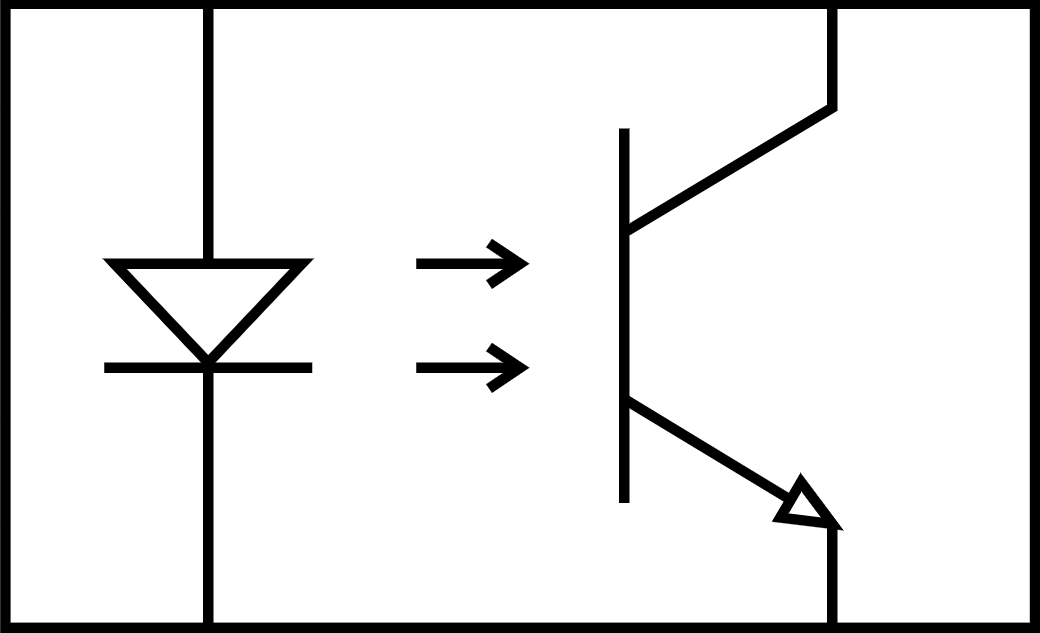
\includegraphics[width=\textwidth/4]{03-placa/02-optoac.png}
    \caption{Ejemplo de optoacoplador}
    \label{fig:figura32}
    \end{figure}

\subsection{Optoacopladores}

En la figura \ref{fig:figura33} se muestra el circuito empleado. Se toman las señales de 24V

\begin{figure}[hbtp]
    \centering
    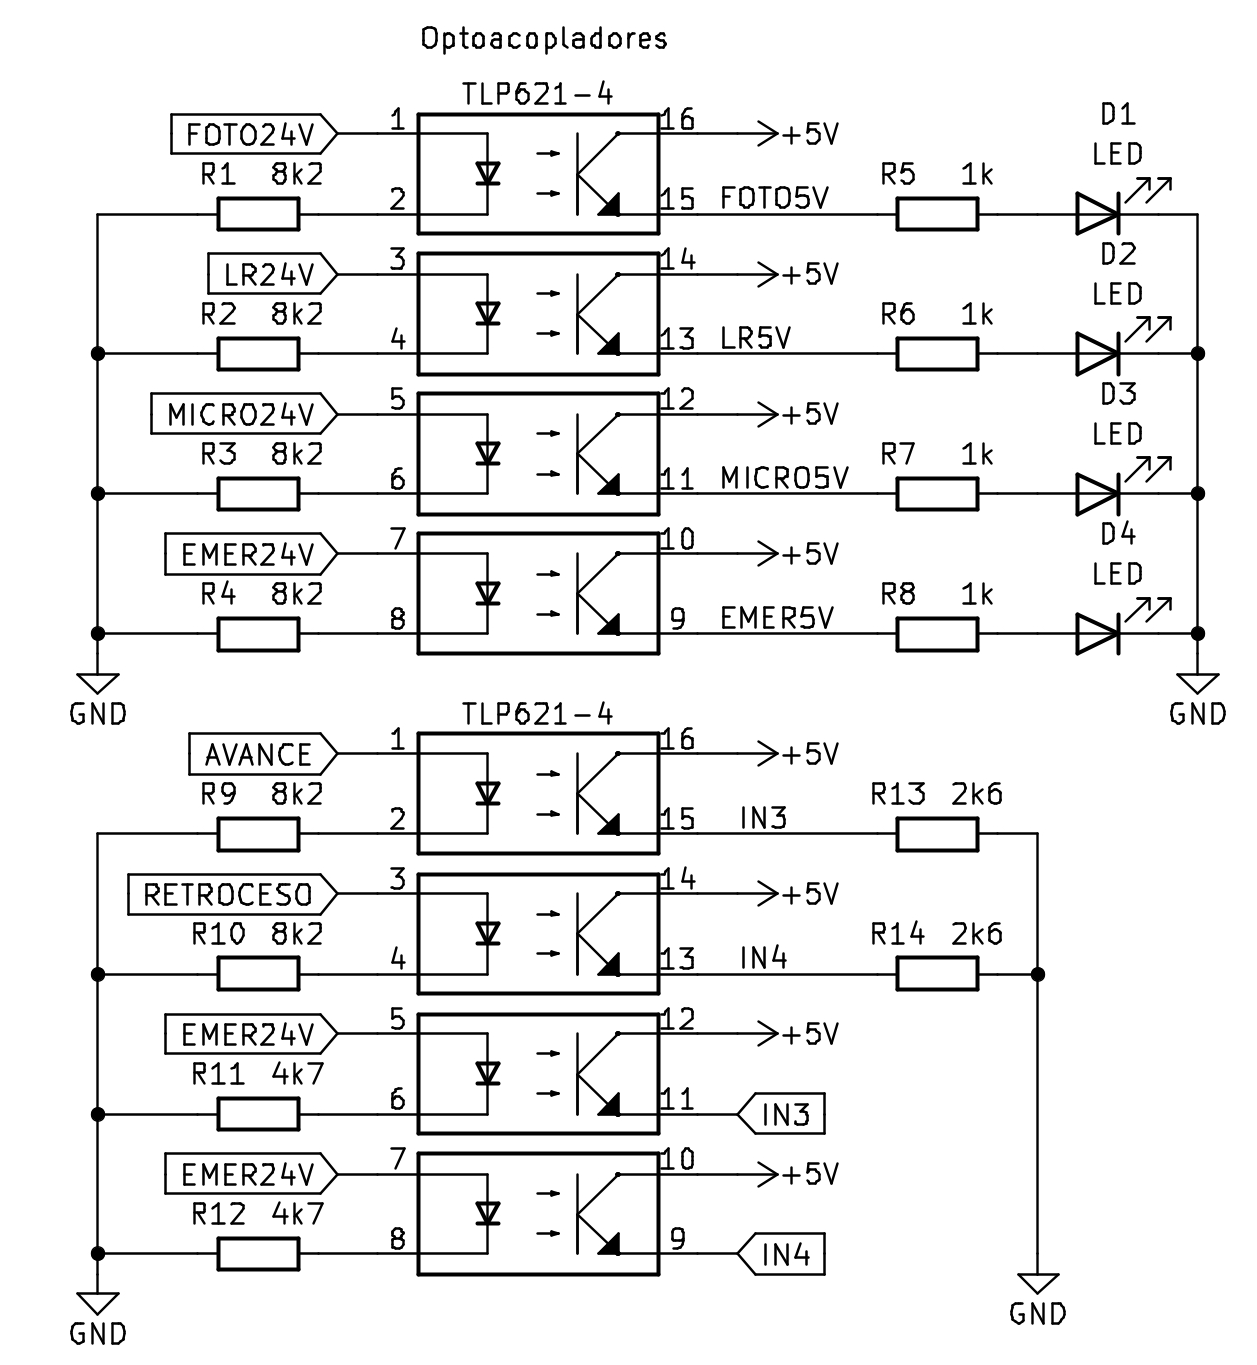
\includegraphics[width=\textwidth/2]{03-placa/03-optoacopladores.png}
    \caption{Ejemplo de optoacoplador}
    \label{fig:figura33}
    \end{figure}


Calibre digital
Tapa
